\documentclass{article}

\usepackage[margin=1in]{geometry}

\usepackage{hyperref}
\usepackage{graphicx}
\usepackage{wrapfig}
\usepackage{lscape}
\usepackage{rotating}
\usepackage{epstopdf}

\title{The Riscy Processor}
\author{Karan Bavishi, Mark Mansi, Suhas Pai, Preyas Shah}
\date{}

\begin{document}

\maketitle

\section{Introduction}

We implement the RV64I set of instructions in the RISCV ISA\cite{riscv-isa}
with a superscalar, out-of-order core. Our implementation is optimized for
correctness. Our second goal was performance.  Our third goal was
synthesize-ability.
%All goals have been compromised for the sake of completion.

In Section~\ref{sec:overview}, we provide a brief overview of our design. In
Section~\ref{sec:modules}, we talk about the design of each individual module
in detail. Section~\ref{sec:perf-policies} describes some of the policies we
designed and implemented to boost the performance of our processor. In
Section~\ref{sec:design-dec}, we discuss and explain some interesting design
decisions we made. In Section~\ref{sec:design-chal}, we talk about a few
challenges that we ran into, which forced us to rethink portions of our design.
Finally, in Section~\ref{sec:performance}, we discuss the performance achieved
by our processor for certain benchmarks, along with some key take-away points
we learned by our experience.

\section{Overview}
\label{sec:overview}

\begin{itemize}
    \item 4-wide pipeline
    \item Out-of-order execution; In-order commit
    \item Fetch (3 cycles for cache hit)
        \begin{itemize}
            \item Branch prediction (TODO): 2-level predictor, BTB, global
                history register.
            \item I-Cache: Blocking, 4 KB, 2-way associative, 1 read/write
                port, 2-cycle latency.
            \item Prefetch Buffer: 4 entries, 32 bytes each
        \end{itemize}
    \item Decode and Rename (2 cycles)
        \begin{itemize}
            \item 64-entry ROB
        \end{itemize}
    \item Issue and FUs (3 cycles)
        \begin{itemize}
            \item 4 ALUs
            \item 4 issue queues, 16 entries each, 1 ALU per queue
            \item Load-balancing arbiter places new instructions in issue
                queues.
            \item ALUs also used to compute \texttt{ld}/\texttt{st}/branch
                addresses.
        \end{itemize}
    \item Address Queue
        \begin{itemize}
            \item 32 entries
            \item Tracks load/store dependencies.
            \item Non-speculative memory disambiguation.
            \item Loads access cache out-of-order between stores.
            \item Stores access cache on commit.
            \item D-Cache (TODO)
        \end{itemize}
    \item Writeback (2 cycle)
        \begin{itemize}
            \item Processor supports back-to-back execution of dependent
                instructions.
            \item Writeback structure (a.k.a ROB WB or more affectionately,
                \texttt{FooPP}) is designed to avoid the massive tangle of wires
                created by broadcast-based writeback among 4 ALUs and a LSQ.
        \end{itemize}
    \item Commit (1 cycle)
    \item Stall: we implement a distinct top-level module to handle stall
        coordination among all stages. The two stall producers in the pipeline
        are the issue queue arbiter and the ROB. A stall is generated when there
        is not enough room in the issue queues or the ROB. Each stage is a
        consumer of stalls produced by stages before it.
\end{itemize}

\begin{figure}[ht]
	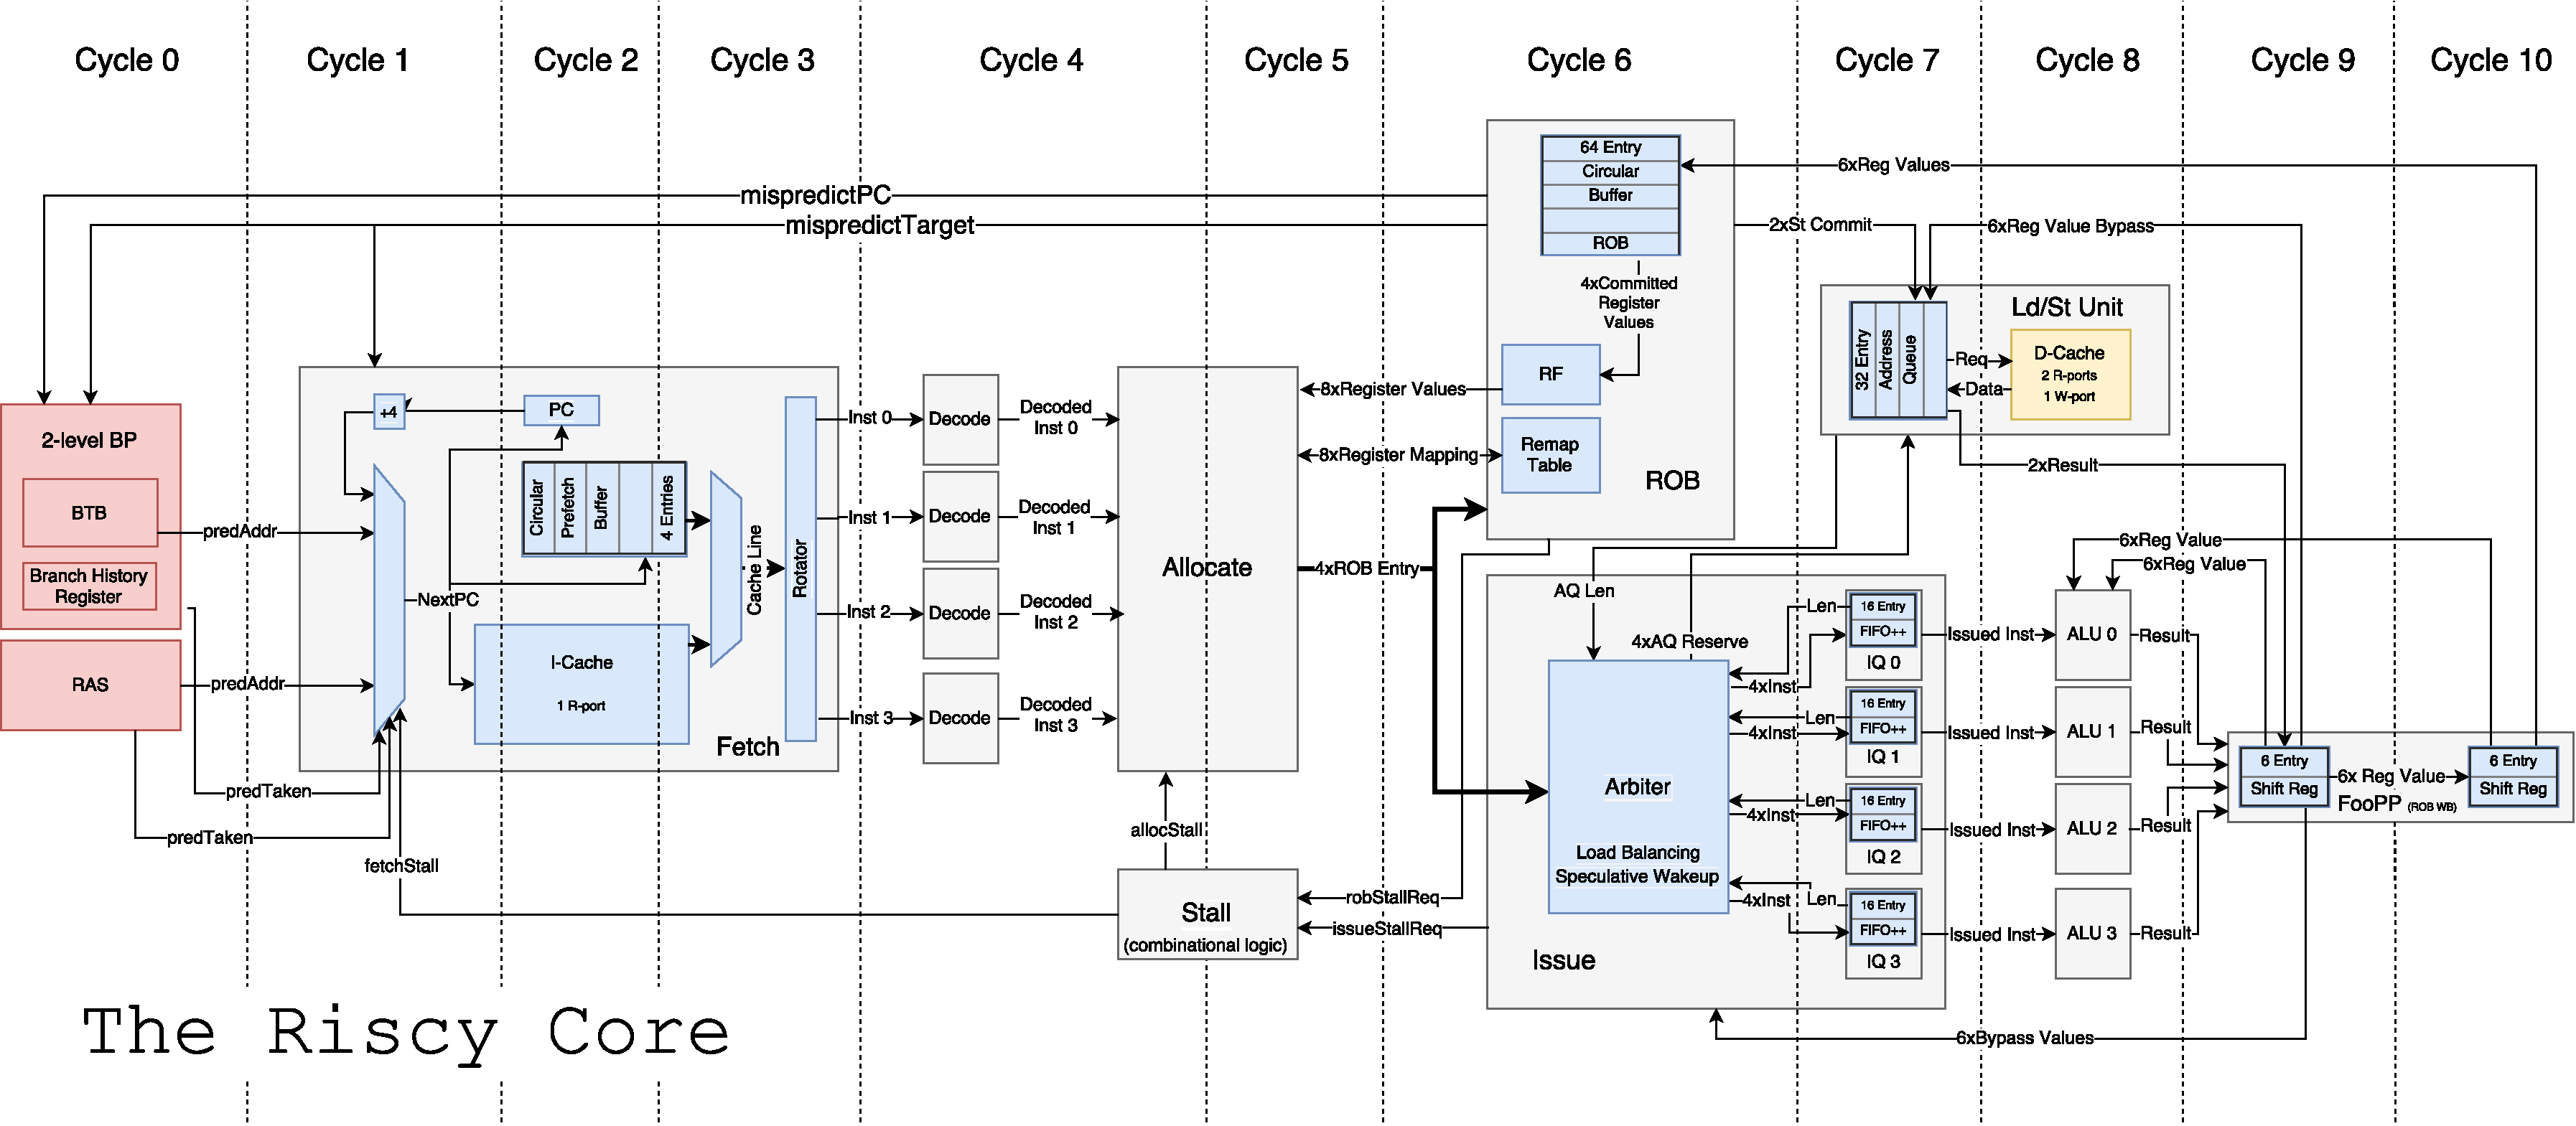
\includegraphics[page=1,width=\textwidth]{riscy_diagram.pdf}
    \caption{\textit{Top-level diagram of our processor} A larger version of
    the diagram is also available at \cite{riscy-diagram}.}
	\label{fig:top-level}
\end{figure}

\section{Modules}
\label{sec:modules}

Our processor has an 11 cycle pipeline depth, as shown in Figure
\ref{fig:top-level}. The pipeline is divided into several independently
designed and implemented blocks (implemented as modules in Chisel). This
section presents an overview of each block.

\subsection{Fetch}

Our fetch module encapsulates the logic of selecting the next PC, issuing
requests to the instruction memory hierarchy (including the I-cache), and
presenting raw instructions to the subsequent stage (decode).

We implement a pipelined, blocking, 2-way associative instruction cache with
2-cycle latency. An additional cycle of latency comes from computing the next
PC.

The instruction cache returns a hit if it finds the requested entry. If not, it
issues a refill request to memory for the missing address. Once the memory
responds, it refills its data and tag arrays with the response. The cache line
replacement policy is random replacement.

We also added a prefetch buffer, containing 4 entries. It does cache block
prefetching; i.e. it stores the additional cache lines sent by memory as a part
of its response to a refill request. This is primarily done to get around the
single-port limitation of the I-cache. This prefetch buffer can be easily
changed to do next-line prefetching as a part of future work.

The output from the instruction cache is rotated and presented to the rest of
the pipeline.

\subsection{Decode and Allocate}

The next two cycles decode and rename the instructions from fetch.

Decode takes less than one cycle because it contains no logic (it just separates
wires). Thus, we combine decode with the first cycle of renaming.

Renaming proceeds in two phases. The first renames all destinations. This can be
done regardless of which instruction is being renamed because all instructions
get a single ROB entry. The second cycle renames operands and produces an ROB
entry which can just be latched to the ROB next cycle. Renaming operands
requires the knowledge of the renamed destinations and previous remappings from
the remap table. Producing an ROB entry, requires reading the register file and
ROB because our design is read-before-issue.

\subsection{ROB}

The ROB is implemented as a 64-entry circular buffer.  We choose to use an ROB
as opposed to a merged register file because we prioritized performance and ease
of implementation over energy.  It serves a few major roles in the pipeline.

\begin{enumerate}
    \item It serves as a central location of information about instructions
        currently in the pipeline, including operands, renaming information, and
        written-back values. Thus, the ROB must be read by Allocate stages to
        produce new ROB entries. In any given cycle, up to 4 new instructions
        may be entered into the ROB.

    \item It is responsible for updating the architectural state when an
        instruction commits, including updating registers and notifying the L/S
        Unit that a store should go to memory. Up to 4 instructions can commit
        in a cycle, including up to 2 store instructions.

    \item It serves as a point of serialization for instructions to commit in
        order. This preserves interruptability and allows recovery from
        mispeculations.

    \item It notifies the rest of the pipeline when a mispeculation happens and
        is responsible for communicating to other modules which instructions in
        the pipeline are valid. It also notifies fetch and the branch predictor
        of the correct branch target.
\end{enumerate}

\textbf{Eras} To aid with identifying squashed instructions, the ROB keeps track
of the mispeculation \textit{era}. New instructions coming into the pipeline are
deemed to be part of the current era. When a mispeculation occurs, a new era
begins.  Instructions in the pipeline are uniquely identified by their ROB entry
number and tag. These values are propagated through the pipeline with the
instruction. The ROB also provides the current era number to other pipeline
stages.

\subsection{Issue and FUs}

In the same cycle, an ROB entry both latches in the ROB and goes to the issue
queue arbiter, which puts it in a queue. All instructions go through the arbiter
regardless of their type. Notably, the issue queues are designed to be largely
oblivious to a number of factors which would have complicated implementation
(and the issue queues are already highly complicated structures). For example,
the issue queues are mostly unaware of the current ROB era and even of
instructions' opcodes.

Our issue stage consists of an arbiter feeding 4 issue queues.
The arbiter does load balancing to attempt to keep any queue from becoming
filled while other ALUs are available.

Each issue queue is independent and feeds a single ALU. The issue queues can
each independently wake up a single instruction to be sent an ALU. Our
implementation is capable of speculatively waking up ALU operations when their
operands are known to be nearly ready. This allows our processor to execute
instruction with back-to-back dependencies. Our writeback mechanism helps with
this also...

\subsection{Writeback}

Each cycle, our processor may produce up to 6 values that need to be written
back (4 from ALUs and 2 from memory). To avoid creating $O(n^2)$ wires between
all of these value producers/consumers, we designed a central writeback
structure, which we call \texttt{FooPP}. All values are written to the
\texttt{FooPP} in the cycle they produced. Any consumers of those values,
including the ROB, issue queues, and L/S Unit, take the values directly from the
\texttt{FooPP}.

To avoid adding a 1 cycle bubble between instructions with back-to-back
dependencies, the \texttt{FooPP} keeps 1 cycle of history, which the FUs can
then consume from easily.

The writeback structure also filters out any values coming from squashed
instructionsby comparing the era of the input values with the current ROB era
number. This allows us to get rid of the squashed instructions easily by letting
them percolate through the pipeline.

\subsection{Load/Store Unit}

When a load or store instruction reaches the arbiter, the arbiter asks the
address queue to reserve a spot for it. If the address queue is full, the
pipeline stalls. The arbiter then puts the load or store in a normal issue queue
to wait until an ALU can compute its address. When the address is written to the
\texttt{FooPP}, the address queue will consume it.

Loads can access the D-cache as soon as their address is known and it is also
known that there is no preceding store to the same address. Stores can access
the D-cache as soon as the ROB signals the address queue that they have
committed.

To limit the number of ports need on the D-cache, we assume only two ports. The
ROB gives the guarantee that no more than 2 stores will commit in any cycle.

\section{Performance Enhancement Policies}
\label{sec:perf-policies}

In this section, we talk about some of the design decisions we took which were
aimed at improving the performance of our processor.

\subsection{Fetch}

We added a prefetch buffer which stored cache blocks when a refill response was
received from memory. This helped us get around the limitations of having a
single-ported I-cache, which allowed us to only write one cache line when the
refill response was received. Having a prefetch buffer allowed us to store
multiple cache lines.

The prefetch buffer also helped improve performance by having enough
instructions to keep the backend busy. Without the prefetch buffer, we were only
able to serve instructions every 2 cycles before incurring another hit.

\subsection{Decode and Allocate}

Decode is combined with the first stage of Allocate to avoid wasting a cycle.

\subsection{ROB}

In case of a misprediction, there are two ways to squash the speculated
instructions. The first involves adding valid bit wires everywhere, and
resetting them when a misprediction occurs. The second way is to let the
squashed instructions percolate through the pipeline normally and ignore the
result. We chose the second approach in our design.

However, the ROB cannot latch new instruction unless all the squashed
instructions have been flushed from the system because ROB entry numbers would
cease to be unique (a correct instruction and a squashed instruction may alias).
Thus, we add misprediction eras. As stated previously, Whenever ROB realizes a
misprediction, it increments the era counter, so squashed instructions are those
from previous eras.

This allows our pipeline to begin execution of correct instructions before the
pipeline is fully flushed.

\subsection{Issue}

Renamed instructions are sent to both the ROB and Issue modules in parallel to
save a pipeline stage.

We also added support for speculative wakeup of instructions whose operands
would be ready in the subsequent cycle. This allowed us to perform back-to-back
execution for dependent instructions and boost performance. (At the moment, we
only support speculative wakeup for ALU operations, but this logic can be
extended for memory loads, too).

\subsection{Execute}

The \texttt{FooPP} module is also responsible for storing the results for 2
cycles for bypass. This bypass support allowed us to execute dependent
instructions in back-to-back cycles.


\section{Design Decisions}
\label{sec:design-dec}
In this section, we talk about the interesting design choices we made for our
processor.

\begin{enumerate}
	\item Pipelined Decode \& Rename - In our Decode and Allocate design,
	we decode and rename the destination in the first cycle.  Renaming of
	operands is done in the second cycle. This allows us to allocate new
	entries in the ROB in the second cycle, in parallel with the renaming
	of operands.

	\item Use Writeback to flush values from squashed instructions - As
	mentioned in Section~\ref{sec:perf-policies}, we decide to let the
	instructions to be squashed percolate through the pipeline.  An
	interesting question was to how to filter out the results from these
	squashed instructions and not make them be mistakenly used for bypass.
	We ultimately decided to add some filter logic to the Writeback module
	inputs. This made sure that the squashed values were invalidated and
	thus never available for bypass.

	\item Arbiter load-balancing and bypass - Our original idea was to have
	the arbiter build dependency graphs and put dependent instructions in
	the same queue. The rationale was that putting dependent instructions
	in the same queue would reduce the overhead of bypass across queues.
	However we soon realized that this plan would result in a multi-cycle
	arbiter design.

	We ultimately decided to have a simple arbiter which would issue
	instructions based on load balancing, i.e. instructions would be issued
	based on the emptiness of the queues. This allowed us to design a
	single-cycle arbiter. However, this brought back the original problem
	of complex bypass. For this, we designed the Writeback structure which
	would allow bypass of computed values to the 4 ALUs.

	\item LSQ: Use Issue queue wakeup logic for load/store instructions -
	Our original plan was to have 4 issue queues and 1 load-store queue,
	using 4 ALUs and 1 AGU. But we decided to re-use the existing ALUs for
	address computation for loads and stores.  This would allow us to
	re-use the complex instruction wakeup logic already present in the
	Issue Queues, and not re-implement from scratch.

	\item LSQ: Serialize loads and stores so that D-cache can have 1 read
	port and 2 write ports - TODO

	\item Unified Stall logic - We decided to come up with a unified stall
	module which would take stall requests as input from ROB and Arbiter
	modules and generate stall outputs to the consumers such as the Fetch
	and the I-cache modules. This unified logic simplified the interface
	between all these modules, and avoided complex wiring.
\end{enumerate}

\section{Design Challenges}
\label{sec:design-chal}
In this section, we talk about certain challenges that we encountered which
forced us to modify our design.

\subsection{Cancelling memory requests}

After adding misspeculation recovery support, we found that our processor had a
5-cycle bubble before instructions were fetched from the new target. On
investigating more, we realized that it was because the I-cache was busy
requesting an address from memory that would no longer be needed.  To get around
this, we added support for cancellation of requests to memory. This required
changes to the memory and I-cache interfaces.

\subsection{ROB deadlock issues}

During testing, we found the processor often entered a state of deadlock. We
realized that we needed to rethink the mean of stalling the ROB. We found that
the ROB should conceptually be though of as two independent modules: allocation
and commit. Allocation should stall. But since commit is the only way for the
processor to make progress, it should never stall.

\subsection{Issue queue timing}

Each issue queue is FIFO-like. Because of writeback and wakeup logic, entries in
the middle of the queue may be woken up and removed or writtenback to and
modified. In addition, an entry may shift while it is being modified. Finally,
the issue arbiter is inserting new entries into the issue queues at the tail.

Because of the high fan-in, we had to carefully design the issue queue logic to
ensure robustness to timing issues. If not done carefully, entries could be
duplicated or lost, fail to be issued or fail to be updated.

\subsection{Zombies}

While adding support for misspeculation recovery through percolation, we
realized that squashed ``zombie'' instructions could end up staying much longer
in the issue queue if their operands not ready.  Consider the case where a
zombie load instruction is kept waiting for 100 cycles waiting for the memory to
respond to the request. This can happen because in our percolation policy, we
execute the zombie instructions but decide to filter the results, simplifying
issue logic.

In order to mitigate this problem, we allow instructions to issue immediately if
they are zombies, even if their operands are not ready. Since we do not care
about the results of these instructions, we allow them to wakeup as soon as an
ALU is available.

\section{Performance}
\label{sec:performance}

\subsection{Methodology}
We ran a series of workloads to show the upper and lower bounds of IPC that our
processor could achieve. We ran the workloads in two main settings to test the
impact of lack of a data-cache and data-prefetching:
\begin{itemize}
\itemsep 0em
	\item 7 cycle memory latency
	\item 4 cycle memory latency (smallest possible latency supported by
	our design)
\end{itemize}

Additionally, we also ran the same workloads with instruction prefetching
turned on. In Section~\ref{sub:results}, we talk about the results achieved
with the two above-mentioned settings, and along with instruction-prefetching
wherever correctness of the benchmarks was verified.

\subsection{Benchmarks}
These are the benchmarks we ran:

\begin{center}
    \begin{tabular}{ | p{1.8cm} | p{1.9cm} | p{1.75cm} | p{5cm} |}
    \hline
    Benchmark & ILP & Instructions & Description \\ \hline
    Counters (optimal) & High ILP & 8K insts & 32 counters incremented
    independently. \\ \hline
    Fibonacci & Max ILP 1.5 & 150 insts & Compute the first 64 Fibonacci
    numbers. \\ \hline
    Daxpy & High ILP (50 \% memory insts) & 3K insts & Element-wise addition of
    arrays. \\ \hline
    Stall (worst case) & Low ILP & 160 insts & Back-to-back dependent
    instructions force in-order execution \\
    \hline
    \end{tabular}
\end{center}

Briefly, here is why we chose each benchmark:
\begin{enumerate}
    \item \textit{Counters} - In this benchmark, we increment 32 counters
        independently. This benchmark has extremely high ILP, so it is optimal
        for a superscalar out-of-order processor. This benchmark reveals the
        upper limit of IPC that can be achieved by our design.

    \item \textit{Fibonacci} - The Fibonacci benchmark is aimed at testing
        our design with a purely compute-based workload. Due to the
        dependencies in the Fibonacci recurrence relation, the maximum ILP that
        can be achieved is 1.5 IPC.

    \item \textit{Daxpy} - We use a loop-unrolled version of the DAXPY
        benchmark. Since the original version involves multiply instructions
        which are not supported in our design, we simply add instead. This
        benchmark has a high ILP workload with a high memory-to-compute ratio
        (50\%) of instructions. This benchmark shows how much the lack of
        data-caching affects our performance.

    \item \textit{Stall} - In this benchmark, we execute 160 back-to-back
        dependent instructions. The maximum ILP that can be achieved is 1. This
        benchmark verifies that our design can execute dependent instructions in
        back-to-back cycles with no bubbles.
\end{enumerate}

\subsection{Results}
\label{sub:results}

In the following table, we describe the IPC achieved for all the benchmarks in
the 2 chosen memory latency settings, with instruction prefetching enabled and
disabled. We omit results for settings where we were unable to verify
correctness.

\begin{center}
    \begin{tabular}{|l|c|c|c|c|}
    \hline
    Setting & Counters & Fibonacci & Daxpy & Stall \\ \hline
    7 cycle, I-prefetch disabled & 0.80 & 0.74 & 0.80 & 0.74 \\ \hline
    7-cycle, I-prefetch enabled & 2.22 & 1.30 & - & 0.91 \\ \hline
    4 cycle, I-prefetch disabled & 1.14 & 1.04 & 0.88 & 0.92 \\ \hline
    4 cycle, I-prefetch enabled & 2.66 & - & - & - \\
    \hline
    \end{tabular}
\end{center}

The following interesting observations can be made:
\begin{enumerate}
    \item \textit{Instruction prefetching makes a huge difference}. As shown by
        the IPC of the best-case Counters benchmark, it is hard to achieve a
        high throughput unless you have enough instructions to keep the backend
        busy. With instruction prefetching disabled, our processor incurs the
        memory latency penalty every 2 cycles.

        Interestingly, even with prefetching enabled, our design is only able
        to reach an ILP of 2.66. The reason for this is that our prefetching
        design is fairly naive; it is not even a next-line prefetcher. The
        prefetch unit does not fetch instructions well in advance and only
        stores additional cache lines when a penalty is incurred. If we
        increase the size of the prefetch buffer from 4 to 8, our projections
        show that we can achieve an IPC of about 3.2.

        Having a more intelligent prefetcher and increasing the size of the
        prefetch buffer should help boost the IPC close to the maximum
        theoretical limit of 4.

    \item \textit{It is important to have a big instruction window}. Similar to
        our previous observation, it is extremely important to have a big
        instruction window to exploit the techniques implemented in an
        out-of-order design. Without enough instructions in the frontend, it is
        difficult to find enough ILP, and the processor remains hampered by
        dependencies and memory latency.

    \item \textit{Memory latency can significantly degrade the IPC}. As can be
        seen from the IPC numbers achieved by the Daxpy benchmark, it is hard to
        achieve a high ILP unless the memory latency can be hidden effectively.

        The Daxpy benchmark has an inherently high-ILP workload, but since our
        design lacks a data-cache, it is unable to go beyond executing more than
        one instruction per cycle.

    \item \textit{Close to optimal performance in Fibonacci} - We achieve an ILP
        of 1.30 for the 7-cycle, prefetching enabled setting, which is quite
        close to the theoretical limit of 1.5. We can actually reach an even
        higher figure of 1.42 for the 4-cycle, prefetching enabled setting, but
        we decided not to show it here because we couldn't get the correct
        result from the benchmark.

    \item \textit{We have near optimal performance in Stall}. Our Stall
        benchmark results are very close to the optimal IPC of 1. This
        highlights our processor's ability to execute dependent instructions in
        back-to-back cycles with no bubbles.
\end{enumerate}


\begin{thebibliography}{9}

\bibitem{riscv-isa} RISCV ISA -  \url{https://riscv.org/specifications/}.

\bibitem{riscy-diagram} RISCY Core diagram -
    \url{https://github.com/mark-i-m/riscy/raw/master/riscy/doc/riscy_diagram.pdf}


\end{thebibliography}

\end{document}
